% !TeX program = pdflatex
% !BIB program = biber
\section{Simulation Study}
\label{sec:sim_study}

% Esta seccion es basicamente replicar Fithian and Hastie

% For the following simulations, the data generation process follows a different Gaussian distribution depending the value of $Y$, specifically, $X \mid Y=y \sim N\left(\mu_y, \Sigma_y\right)$. For example, if $Y=1$, then $X \sim N\left(\mu_1, \Sigma_1\right)$, and if $Y=0$, then $X \sim N\left(\mu_0, \Sigma_0\right)$. The level of overlapp (or conditional imbalance?) is dictated on how much $\mu_1$ differs from $\mu_0$.\\

In this section, I compare the performance of CC, WCC, and LCC methods as in \textcite{hastie2014}. Furthermore, I conduct numerical exercises to show the main statistical properties of the LCC method, particularly its asymptotic variance behavior as a scalar of $\Sigma_{full}$. Additionally, I expand on the author's analysis by varying the data generation process (DGP) in the last two simulation exercises to examine the methods' performance on different population sample sizes $N$ and various levels of marginal imbalance.\\

To the best of my knowledge, there are currently no available R packages to implement the algorithms as presented in Section \ref{sec:Methods}. Thus, I developed and wrote the functions for their application and usage using R Statistical Software, version 4.2.1 (\cite{R}). All functions, simulation exercises, analyses, plots, and figures shown here can be accessed for review and reuse at \href{https://github.com/carolinalvarez/code-MA-thesis}{https://github.com/carolinalvarez/code-MA-thesis}. Additionally, some of the color palettes for the figures generated were taken from \textcite{wesanderson}.

\subsection{General setup}
\label{sec:sim_general}

Following mainly \textcite{hastie2014} but also \textcite{wang2020rare} and \textcite{han2020local}, the regressors in the general DGP follow a different Gaussian distribution depending on the value of $Y$. That is, $X \mid Y=y \sim N\left(\mu_y, \Sigma_y\right)$. If $Y=1$, then $X \sim N\left(\mu_1, \Sigma_1\right)$, and if $Y=0$, then $X \sim N\left(\mu_0, \Sigma_0\right)$. The imbalanced ratio or degree of marginal imbalance is set by $P(Y=0) = r$, implying $P(Y=1) = 1-r$. Furthermore, assume the data also has conditional imbalance, generated by creating a specific set in $\mu_1$ where $P(Y=1 | X = \mu_1) \approx 1$. Thus, let $\mu_0$ and $\mu_1$ be defined as:

\begin{equation}
    \nonumber {\mu}_0=[\underbrace{0,0, \ldots, 0}_{k}]^{\prime},
    {\mu}_1=[\underbrace{0,0, \ldots, 0}_{\frac{k}{2}}, \underbrace{1,1, \ldots, 1}_{\frac{k}{2}}]^{\prime},
\end{equation}

where it is expected that the conditional imbalance increases as $k$ gets larger. For all simulations, the model is correctly specified. Thus, the variance-covariance matrices are set to be identical between the classes, that is, $\Sigma_0 = \Sigma_1$. 

\[
	\mathbfup{\Sigma_1} =
	\mathbfup{\Sigma_0} =
	\mathup{Cov}(X) =
	\begin{bmatrix}
		\mathup{Var}(x_1)      & \cdots & \mathup{Cov}(x_1, x_n) \\[-2.5pt]
		\vdots                 & \ddots & \vdots                 \\
		\mathup{Cov}(x_n, x_1) & \cdots & \mathup{Var}(x_n)
	\end{bmatrix} =
	\begin{bmatrix}
		1      & \cdots & 0 \\[-2.5pt]
		\vdots                 & \ddots & \vdots                 \\
		0 & \cdots & 1
	\end{bmatrix}
\]
\\

Any population size can be drawn from the above setup by setting the desired values of $N, k, \text{and } P(Y=1)$. Additionally, Lemma 1 holds in this setup, indicating a non-separability of classes within the general DGP. To demonstrate this, let's consider a data realization from Simulation \ref{sec:sim1}. Figure \ref{fig:pca1} shows a Principal Components Analysis (PCA) plot of the generated population, where a separation between classes is observed, primarily due to the conditional imbalance present in the data. However, the classes cannot be perfectly separated by a hyperplane, as there is some overlap between the two data clusters.


\begin{figure}[ht]
   \centering
   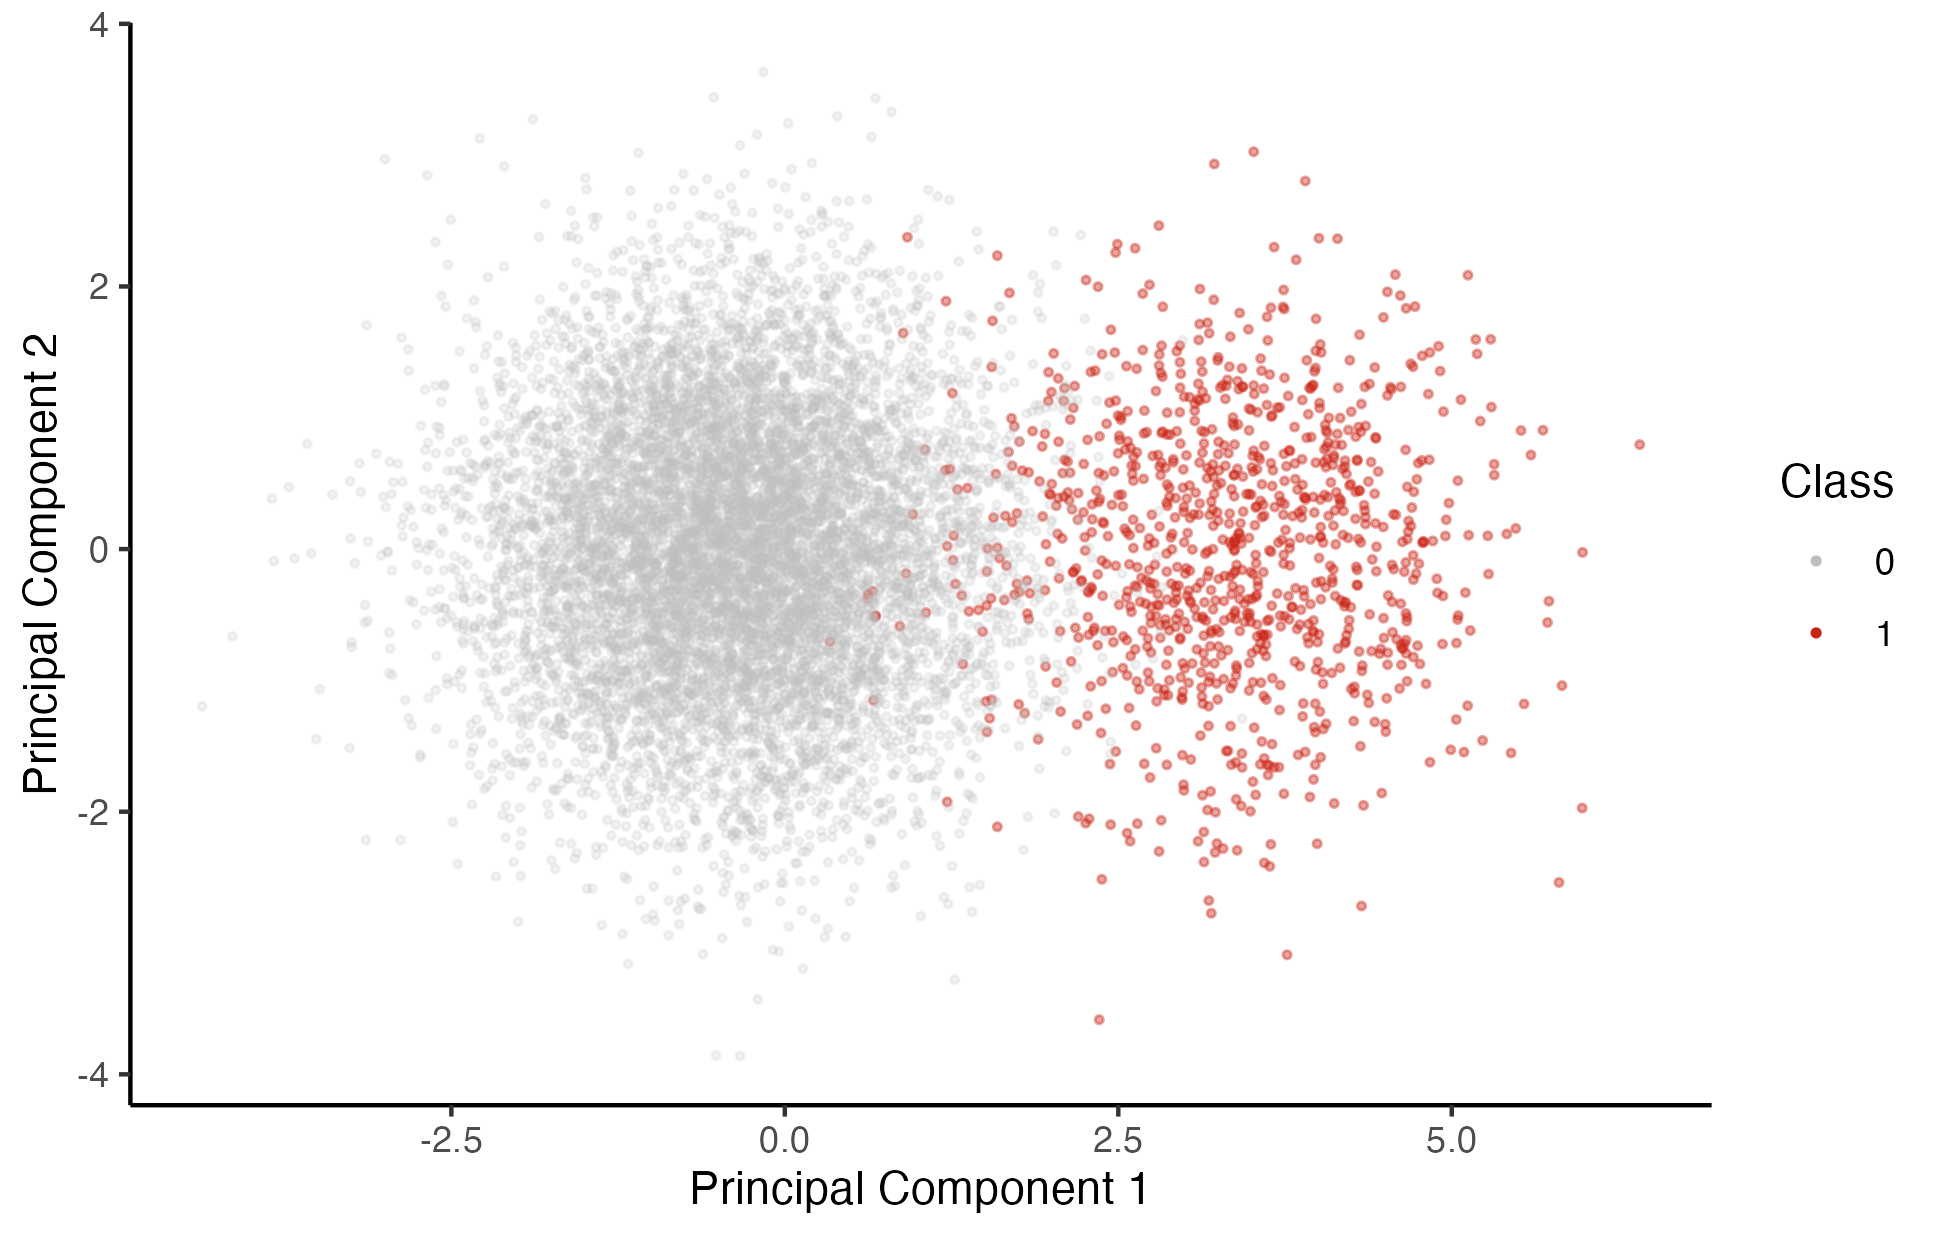
\includegraphics[scale=0.6]{2_Figures/plot_pca_1.png}
   \caption[PCA plot (DGP example)]{PCA plot of example population in Simulation \ref{sec:sim1} showing non-separability of classes.}
   \label{fig:pca1}
\end{figure}


\subsection{Simulation 1}
\label{sec:sim1}

The first simulation closely follows the setup in simulation $2$ of \textcite{hastie2014}. The main idea is to ``replicate'' as closely as possible the findings in the original paper and check whether the R functions for applying the algorithms work as intended. Since the linear model is correctly specified, all methods are asymptotically unbiased; therefore, the exercise is meant to show the superiority of the LCC method in terms of the variance of the model.\\

Let the size of the population be $N=10^5$, the marginal imbalance in the population $P(Y=1) = 0.1$, the number of regressors $k=30$, $\mu_1=(\begin{array}{l}1_{15}, 0_{15}\end{array}), \mu_0=0_{30}$, and $\Sigma_0=\Sigma_1=I_{30}$ as in Section \ref{sec:sim_general}. To fit the methods, I set the acceptance probability to $a(1)=0.9$ for CC, WCC, and the pilot, so there is a 50-50 split between the classes in the subsample. Since the pilot is taken from a subsample of the full data, it is a data-dependent pilot, as an observation $i$ can be observed by the pilot and LCC model. However, we can expect the LCC estimate still be consistent, as the independence of the pilot is not required for consistency of the estimate.\\

For comparison between the algorithms, the authors fix the subsample sizes, letting CC and WCC have exactly twice as many data points as LCC alone (in this sense, LCC must ``pay" for its pilot, where the latter gets the same amount of data points as LCC). Since the paper does not explicitly show how the authors fix $N_s$, I first run $100$ simulations, fit the methods, store the subsample size $N_s$ for LCC, and approximate the LCC's fixed $N_s$ by roughly taking the median from the $N_s$ realizations. In order to closely follow the authors, I round the LCC $N_s$ to its nearest thousand, and then I fix the CC and WCC subsample sizes as twice the $N_S$ size for LCC. The tables with the median LCC's subsample size used as a reference can be found in Appendix Section \ref{app:summary-stats-Ns} for all simulations.\\

% The results of the simulation study are shown in Table \ref{tab:sim1} and Figure \ref{fig:violin_int_e}. The findings are in line with the results in the original paper; LCC has the lowest bias and variance among the three algorithms. In general, it is a flattering setup for the LCC algorithm: the population sample is very large, and so is the level of both marginal and conditional imbalance. According to the authors, the reason why LCC outperforms CC in terms of variance is that the traditional case-control method cannot exploit the high conditional imbalance in the sample. On the other hand, WCC shows both the largest bias and variance among all methods. Since the method is only asymptotically unbiased, it can be that the fixed size $N_S$ does not allow it to approach its asymptotic behavior. As for the variance, recall that WCC's main drawback is its high variance as a result of variation in the weights. In this setup, as the imbalance is quite large, a large efficiency loss is observed.

Table \ref{tab:sim1} and Figure \ref{fig:violin_int_e} illustrate the simulation study's findings, which support the original paper's results. The LCC algorithm exhibits the lowest bias and variance among all three algorithms. This result is not surprising given the large population sample and high levels of marginal and conditional imbalance in this setup. According to the authors, LCC outperforms CC in terms of variance because traditional case-control methods have no way to exploit conditional imbalance. On the other hand, WCC exhibits the largest bias and variance. As for the bias, it could be that the fixed size of $N_s$ may be too small to allow the method to reach its asymptotic bias behavior fully. Additionally, recall that WCC's main drawback is its high variance as a result of variation in the weights; in this setup, as the imbalance is quite high, a large efficiency loss is observed.

\begin{table}[ht]
    \centering
    \begin{tabular}{lccc}\toprule
        & \multicolumn{1}{c}{$N_s$} & \multicolumn{1}{c}{$\widehat{bias^2}$} & \multicolumn{1}{c}{$\widehat{var}$}
        \\\midrule
        CC  & 4000 & 0.25  & 0.68 \\
        WCC & 4000 & 1.02 & 1.27 \\
        LCC & 2000 & 0.006 & 0.18 \\
        \bottomrule
    \end{tabular}
    \caption[Simulation 1 - Baseline numerical exercise]{Simulation 1 - Baseline numerical exercise (results for 1,000 runs).}
    \label{tab:sim1}
\end{table}


\begin{figure}[ht]
    \centering
    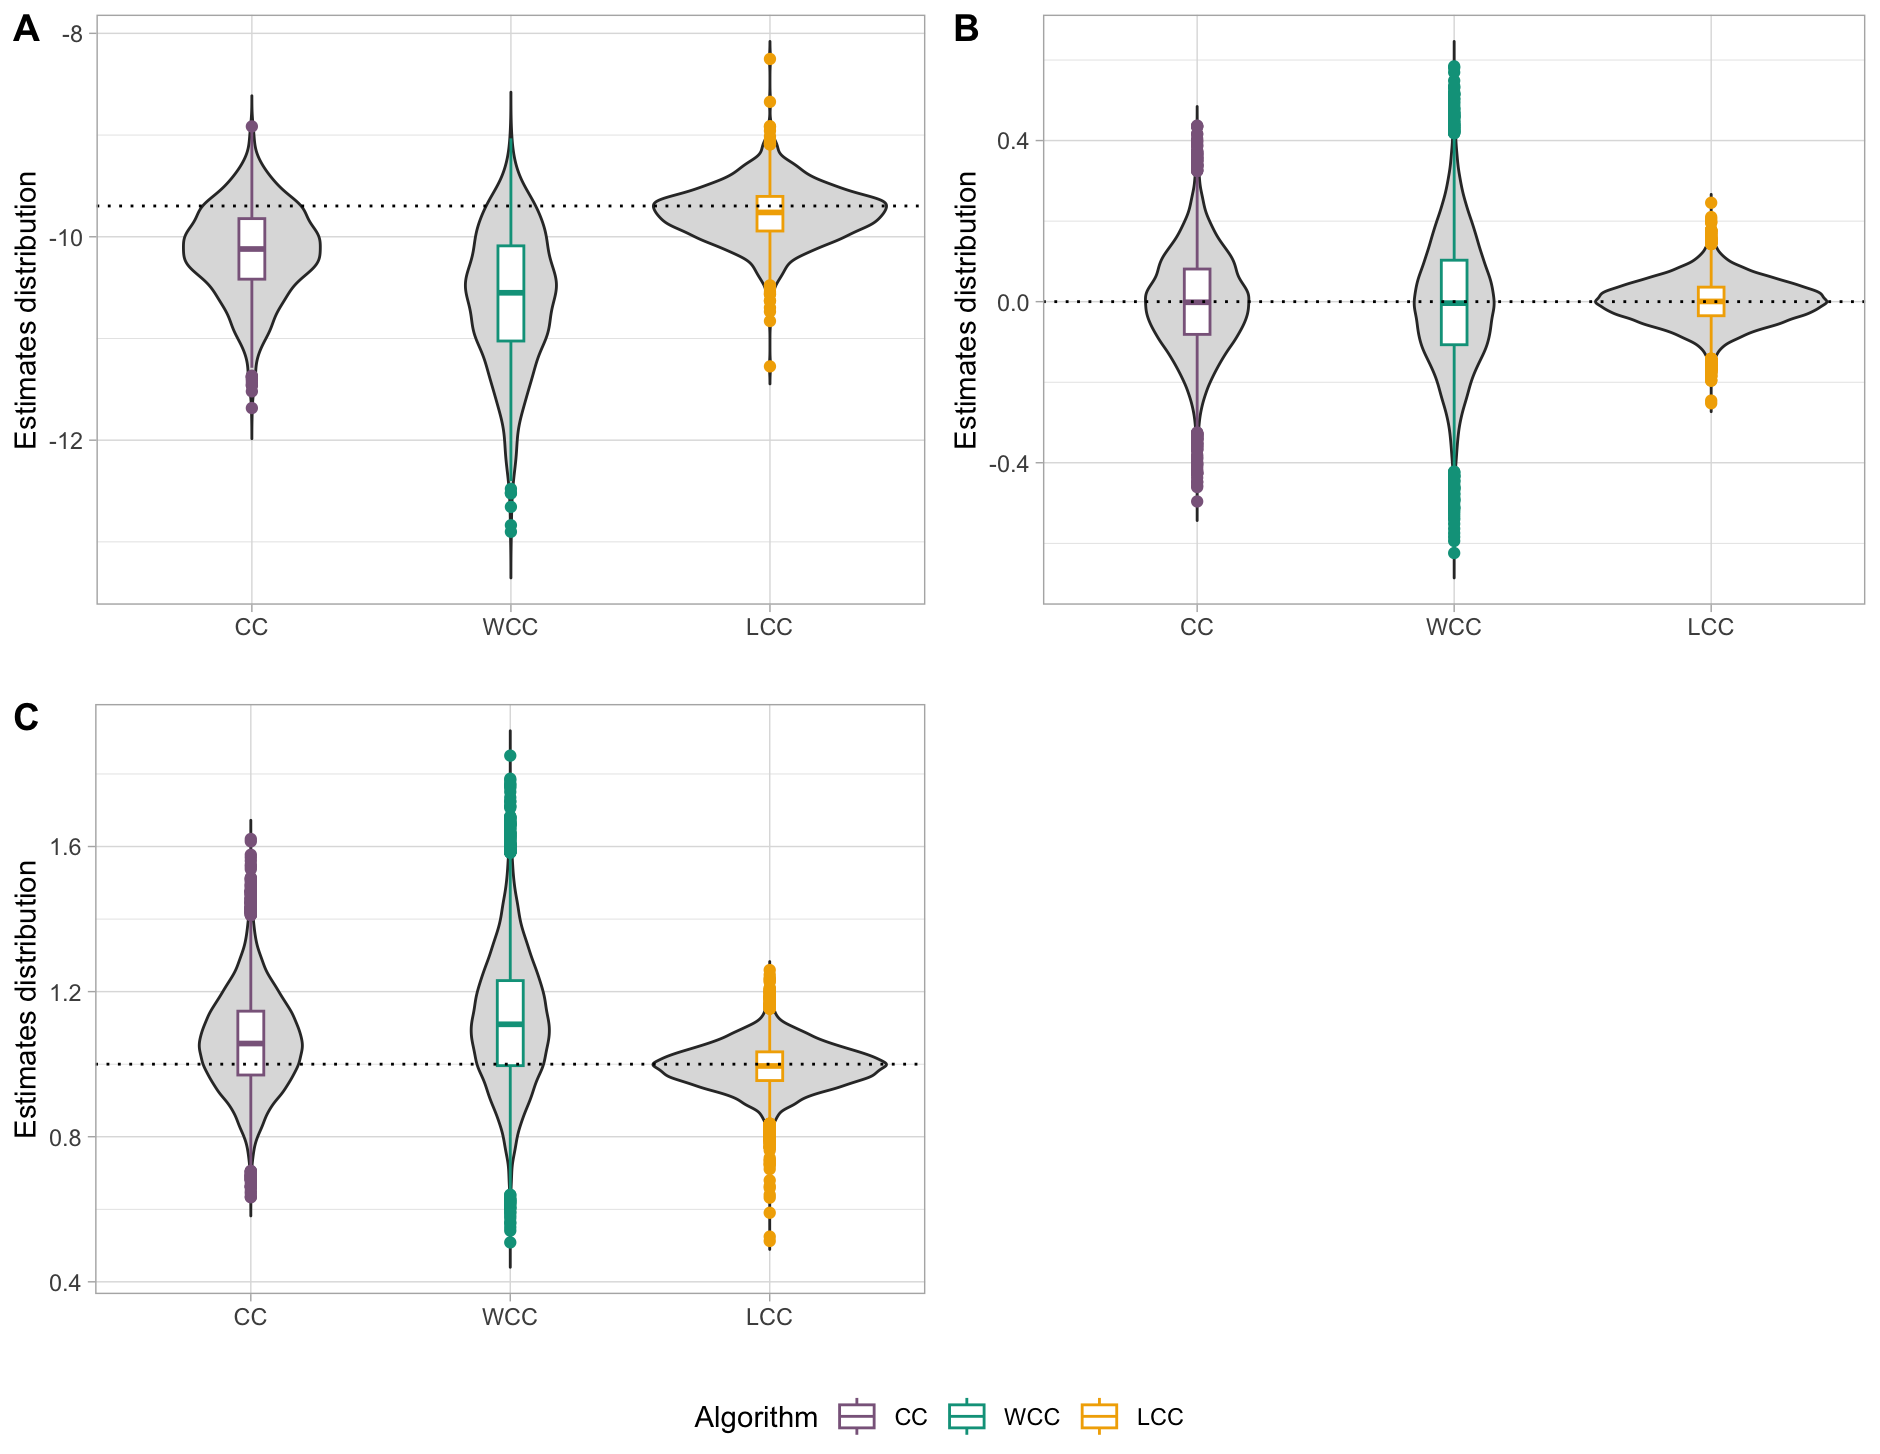
\includegraphics[width=\textwidth]{2_Figures/all_violins2.png}
    \caption[Simulation 1 - Distribution of Monte Carlo realizations $\hat{\theta}_{CC}$, $\hat{\theta}_{WCC}$ and $\hat{\theta}_{LCC}$]{Simulation 1 - Distribution of $\hat{\theta}$ estimates across subsampling algorithms, where the dotted line corresponds to the true parameters' values.
    \textbf{Panel A:} Distribution of intercept coefficients with true $\alpha= - 9.7$.
    \textbf{Panel B:} Distribution of slope coefficients with true $\beta=0$, namely $\beta_1, \dots, \beta_{\frac{k}{2}}=0$.
    \textbf{Panel C:} Distribution of slope coefficients with true $\beta=1$, namely $\beta_{\frac{k}{2}+1}, \dots, \beta_k=1$.}
    \label{fig:violin_int_e}
\end{figure}


 